% Kopfzeile beim Kapitelanfang:
\fancypagestyle{plain}{
%Kopfzeile links bzw. innen
\fancyhead[L]{\Large Vorlesung 30 (06.02.2013)}
%Kopfzeile rechts bzw. außen
\fancyhead[R]{}}
%Kopfzeile links bzw. innen
\fancyhead[L]{\Large Vorlesung 30 (06.02.2014)}
%Kopfzeile rechts bzw. außen
\fancyhead[R]{}
% **************************************************
\section*{Das Newton-Verfahren}\label{Newton-Verfahren}
Zur Berechnung von Nullstellen einer Funktion $f: D \to \R, D \subseteq \R$\nl
Voraussetzung: $f$ ist differenzierbar auf $D$\\
Sei $\xi$ eine Nullstelle von $f$, das heißt: $f(\xi)=0$. Sei $x_0$ eine erste Näherung für $\xi$.\nl
\begin{tikzpicture}
\draw[->] (-3,0)--(3,0);
\draw[color=blue,domain=-2.5:2.5] plot (\x, {(0.15*(\x+2.5)^2)-1.5}) (0.662278,0) node {$\bullet$} node[above] {$\xi$};
\draw[color=red,domain=0:2.5] plot (\x, {(1.35*\x)-1.1625}) (0.861111111,0) node {$\bullet$} node[below] {$x_1$};
\draw[dashed] (2,1.5375) node {$\bullet$} node[right] {$(x_0, f(x_0))$} --(2,0) node[below] {$x_0$};
\end{tikzpicture}

\subsection*{Idee}
Die Nullstelle $x_1$ von $T$ ist bessere Näherung für $\xi$ als $x_0$.\nl
Tangente in $(x_0, f(x_0))$: $T(x)=f(x_0)+f'(x_0)(x-x_0)$\\
$T(x)=0 \Lra x=x_0-\frac{f(x_0)}{f'(x_0)}$, sofern $f'(x_0) \neq 0$\nl
Sei $f'(x_0) \neq 0$. Neue Näherung: $x_1:=x_0-\frac{f(x_0)}{f'(x_0)}$\\
Sei $f'(x_1) \neq 0$. Neue Näherung: $x_2:=x_1-\frac{f(x_1)}{f'(x_1)}$\\
usw.\nl
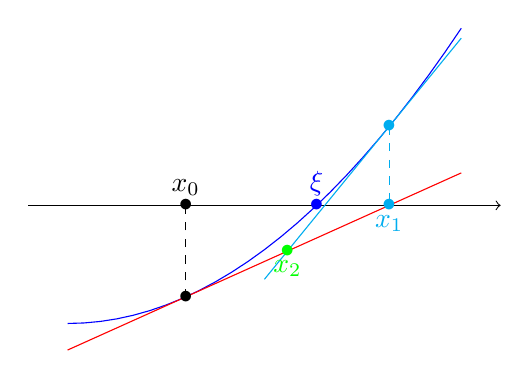
\begin{tikzpicture}
\draw[->] (-3,0)--(3,0);
\draw[color=blue,domain=-2.5:2.5] plot (\x, {(0.15*(\x+2.5)^2)-1.5}) (0.662278,0) node {$\bullet$} node[above] {$\xi$};
\draw[color=red,domain=-2.5:2.5] plot (\x, {(0.45*\x)-0.7125});
\draw[dashed] (-1,-1.1625) node {$\bullet$} --(-1,0) node{$\bullet$} node[above] {$x_0$};
\draw[color=cyan,domain=0:2.5] plot (\x, {(1.224999*\x)-0.93854});
\draw[color=cyan,dashed] (1.58333,1.001037583335) node {$\bullet$} --(1.58333,0) node {$\bullet$} node[below] {$x_1$};
\draw[color=green] (0.291665,-0.581250666665) node {$\bullet$} node[below] {$x_2$};
\end{tikzpicture}

\newpage

\phantomsection
\addcontentsline{toc}{section}{Definition: Newton-Iteration}
\section*{Definition: Newton-Iteration}
$x_{n+1}=x_n-\frac{f(x_n)}{f'(x_n)}$, sofern $f'(x_n) \neq 0, n \in \N_0$

\subsection*{Beispiel}
Sei $a>0$.\\
Gesucht: $\sqrt{a}$ (Näherung dafür)\nl
$f(x)=x^2-a, f'(x)=2x$\\
$x_{n+1}=x_n-\frac{x_n^2-a}{2x_n} = \frac{1}{2} \cdot \left(x_N + \frac{a}{x_n}\right)$ (auch bekannt als Babylonisches Wurzelziehen, \ref{5.11})

\subsection*{Achtung}
Das Newton-Verfahren kann divergieren, die Konvergenz ist abhängig vom Verhalten von $f$ in der Nähe von $\xi$.

\section{Satz}\label{16.1}
Sei $f: [a,b] \to \R$ eine $C^2$-Funktion (d.h.: zwei Mal stetig differenzierbar auf $[a,b]$) mit:
\en{
\item $f$ hat in $[a,b]$ eine Nullstelle: $\xi$
\item $f'(x) \neq 0 \forall x \in [a,b]$
\item $f''(x) \ge 0 \vee f''(x) \forall x \in [a,b]$
\item Die Iterationen $x_1$ zu $x_0=a$ und $x_0=b$ liegen in $[a,b]$
}
Dann gilt:
\enk{
\item $\xi$ ist einzige Nullstelle von $f$ auf $[a,b]$ (direkt aus (1) und (2))
\item Bei beliebigen $x_0 \in [a,b]$ gilt:\\
$x_n \in [a,b] \forall n, (x_n)$ monoton ab $n=1$, und $\lim_{n \to \infty} x_n = \xi$
\item \underline{Fehlerabschätzung}: $m := \min_{x \in [a,b]} |f'(x)| > 0, M: \max_{x \in [a,b]} |f''(x)|$\\
$\Ra |x_n-\xi| \le \frac{M}{2m} \cdot |x_n-x_{n-1}|^2$\\
(Hat man $x_1,\ldots,x_n$ berechnet, so kann man $|x_n-\xi|$ abschätzen)
}

\newpage

\subsection*{Beweis}
Betrachte Fall $f' > 0 \wedge f'' \ge 0$ (weitere drei Fälle analog)\nl
$g(x) := x - \frac{f(x)}{f'(x)}$ ($\blacksquare$), $g' = 1-\frac{(f')^2-f f''}{(f')^2} = f \cdot \underbrace{\frac{f''}{(f')^2}}_{>0}$\nl
$f$ s.m.w., $f(\xi)=0$\\
$\Ra g'(x) = \left\{\begin{array}{l l l} \le 0 & \text{auf} & [a,\xi] \\ \ge 0 & \text{auf} & [\xi,b]\end{array}\right.$\nl
\begin{tikzpicture}
\draw (-2,0) node {$|$} node[below] {$a$} --(2,0) node {$|$} node[below] {$b$};
\draw[color=blue,domain=-2:2] plot (\x, {(0.25*abs(\x^2))+1.5});
\draw[dashed] (-2,1.5) node[left] {$\xi$} --(0,1.5) --(0,0) node[below] {$\xi$};
\end{tikzpicture}\nl
$\Ra g$ hat absolutes Minimum in $\xi$, $g(\xi)=\xi$; (4) $\Ra g(a), g(b) \in [a,b]$\\
$\Ra \xi \le g(x) \le b \forall x \in [a,b]$ (*)\\
$f \ge 0$ auf $[\xi,b] \Ra g(x) \le x$ auf $[\xi,b]$ (**)\nl
Betrachte nun $(x_n)$: $x_{n+1}=g(x_n)$\nl
\underline{Zu 2.}: $x_0 \in [a,b] \underset{\text{(*)}}{\Ra} x_1 = g(x_0) \in [\xi,b]$\\
Ist $x_n \in [\xi,b]$ gezeigt für $n \in \N \Ra \xi \le \underbrace{g(x_n)}_{x_{n+1}} \underset{\text{(**)}}{\le} x_n \le b \Ra x_{n+1} \in [\xi,b]$\nl
Also: Induktion $\Ra (x_n) \subseteq [\xi,b]$ und monoton fallend ab $n=1$\\
$\Ra x_n \to \hat{\xi} \in [\xi,b]$\nl
$x_0 \in [a,b]$ beliebig, $x_{n+1}=g(x_n), n \in \N_0$\\
$(x_n)_{n \ge 1} \subseteq [\xi,b]$ monoton fallend $\Ra \hat{\xi} := \lim_{n \to \infty} x_n \in [\xi,b]$ existiert\\
$\hat{\xi} = \lim_{n \to \infty} x_{n+1} = \lim_{n \to \infty} g(x_n) \underset{g \text{ stetig}}{=} g(\lim_{n \to \infty} x_n) = g(\hat{\xi})$\\
($\blacksquare$) $\Ra f(\hat{\xi})=0 \underset{\text{Teil 1.}}{\Ra} \hat{\xi}=\xi$\nl
\underline{Zur Fehlerabschätzung}: $x_n \neq \xi \Ra \left|\frac{f(x_n)-\overbrace{f(\xi)}^{=0}}{x_n-\xi}\right| \underset{\text{MWS}}{=} |f'(\mu)| \ge m > 0$ ($\mu$ zwischen $\xi, x_n$)\\
$\Ra |x_n-\xi| \le \frac{|f(x_n)|}{m} \forall n$\nl
Abschätzung von $f(x_n)$: Taylorentwicklung von $f$ um $x_{n-1}$:\\
Lagrange (\ref{15.3}) $\Ra f(x_n) = \underbrace{f(x_{n-1})+f'(x_{n-1}) \cdot (x_n-x_{n-1})}_{=0} + \frac{1}{2} f''(\overline{\mu}) \cdot (x_n-x_{n-1})^2$ ($\overline{\mu}$ zwischen $x_{n-1}, x_n$)\\
$\Ra |f(x_n)| = \frac{1}{2} |f''(\overline{\mu})| \cdot |x_n-x_{n-1}|^2 \le \frac{M}{2} \cdot |x_n-x_{n-1}|^2$\\
$\Ra |x_n-\xi| \le \frac{M}{2m} \cdot |x_n-x_{n-1}|^2$ \qed

\newpage

\subsection*{Beispiel}
$f(x)=x-e^{-x} \overset{!}{=} 0$\\
$f(0)=-1<0, f(1)=1-\frac{1}{e} > 0$\nl
$[a,b]=[0,1]$ wählbar, denn:
\en{
\item erfüllt nach ZWS \ok
\item $f'(x)=1+e^{-x} > 0$ \ok
\item $f''(x)=-e^{-x} < 0$ \ok
\item $x_0=0 \Ra x_1 = \frac{1}{2} [0,1], x_0=1 \Ra x_1=\frac{2}{1+e} \in [0,1]$ \ok
}
$m = 1+\frac{1}{e}, M=1$\nl
Konkretes Beispiel: Startwert $x_0 := \frac{1}{2}$ (1. Iteration zu $0$)\\
$x_1 = 0,566311\ldots$\\
$x_2 = 0,567143\ldots$\\
$|x_2-\xi| \le \frac{M}{2m} |x_2-x_1|^2 < 0,5 \cdot 10^{-6}$